\chapter{Website}

Now that we have discussed all the essential components required to create the website for users to purchase the insurance, we will move to discuss about the actual creation of the website. Our website will be based on a single most important principle: Simplicity. The user will never get to see any technical jargon or need to interact with useless webpages going through things that don't matter to them. Our aim is to make the whole process of buying insurance so simple that the user can but the insurance in three clicks and if the flight is delayed, gets his/her payout automatically. 
\\The insurance process will be carried out with a web app that has been up and running on a publicly accessible server, \url{insurance.pythonanywhere.com}. In this chapter we will first go through all the technologies used to create the website and then go through all the components of the website. 

\section{Technologies Used}
There are multiple technologies that go towards making a full fledged user-facing website. We will discuss all the technologies used and the reasons they were used. Apart from blockchain, we won't go deep into any other technology as it will be out of scope of this paper. 

\subsection{Python}
Python is a dynamically scripted language that has become immensely popular in recent times due to its simplicity and huge developer support. For our project, the following two were the criteria on the basis of which Python was selected as the programming language of choice:
\begin{enumerate}
    \item Web frameworks
    \\Python has very popular native web-frameworks such as Django and flask. Both have great documentation and developer support, essential for this project. 
    \item Data science libraries
    \\ Apart from R, python is the language with most support for the data science libraries and a go to choice for data science algorithms implementation. Even though as already mentioned in the previous chapter that our prediction algorithms were created in R, the final implementation of the algorithms has to be in our web framework language. Hence the availability of such algorithms' native implementation in python was a important consideration
\end{enumerate}

\subsection{Flask}
Flask is one of the most popular frameworks in Python. Even though Django is considered to be more mature platform with higher developer support, flask is easier to start with and had everything that was essential to create the website for us. 

\subsection{MySQL}
MySQL was chosen as a default choice as our database wasn't going to be a complex database. 

\subsection{PyCharm IDE}
PyCharm was the Python IDE of choice for the development process as it was a free choice with native support for flask framework. It also has inbuilt support for version control system.

\subsection{Github}
For software version management, Github was chosen for version control, being the most popular git client. The public account was chosen to create the repository, as it was free and the project does not require any privacy features at the moment.

\section{Website Structure}
The structure of the website consists of the separate aspects of the website at the backend that help in creating the website. 
\subsection{User Administration}
The starting point for every user, user administration is responsible for:
\begin{enumerate}
    \item Registering a user
    \item Logging in a user
    \item Maintaining a user session
\end{enumerate}
A Flask library called flask\_login was used to implement the User administration aspect of the website.

\subsection{SQL model}
The SQL model defines the database model that will be used by the website for keeping user records and flight/insurance details. It contains multiple classes that correspond to unique tables in MySQL database. The first class/model defines the table structure of all the important details for the website:
\begin{itemize}
    \item First name
    \item Last name
    \item Email Address
    \item Password
    \item Flight ID
    \item Date
    \item Insurance ID
    \item Blockchain status
    \item Blockchain receipt
    \item Multiple payout amounts for different categories of delays
\end{itemize}

The second class/model defined creates a MySQL table that is used for our autocomplete feature on the website. Our website will only deal with airlines that land in Germany, hence we have to limit the ability of user to enter a limited set of flights. This is done using the autocomplete feature of jQuery. This model contains all the flight details including origin, destination, airline etc. Once a user starts entering flight ID in the Flight ID field, the options are presented from our database using autocomplete function of jQuery. The user is not allowed to enter any other Flight ID. 

\subsection{Forms}
Forms are the flask's rendition of the HTML5 form fields. It creates HTML5 fields but adds input validation to them and makes them easier to use within our webapp. The library used for flask forms is called as WTforms. 

\subsection{Views}
Views are basic functions that explain the framework what to do for each URL. For ex. we have a login URL for which the login view will be called. Create insurance view will call a view function attached to it's URL and so on. What we generally do is import a form to a view function if any user input is required, perform any function if required on the fields and display it to the user.

\subsection{REST API calls}
REST API is a important component of any dynamic web application today. We use the Request module of Python to make a REST API call whenever we require some data from a third party, like weather, flight data or blockchain anchoring.

\subsection{Email Notifications}
The user has to be notified each time an insurance is created as well as when we have the flight status once the flight has landed. The notifications are currently being sent using my gmail address using a python library called \textit{smtplib}. The user details are taken from the user table, with the flight status, if available, from a REST API call. We add the details to a variable and send that variable to gmail's SMTP server with our own user account details.

\subsection{Blockchain}
As discussed in the blockchain chapter, we use Tierion API to hash our data and anchor it to the blockchain. This is done through a REST API call with user data sent as body in a HTTPS POST request. We receive the id of the request as the response which we store as Insurance ID. We use the same insurance ID to get the blockchain receipt once it's anchored to the blockchain.

\subsection{Insurance payout}
We create a script that runs once everyday with help of cron jobs. The aim of the website is to get the flight status of each flight for which we have created an insurance. If it finds out the status of a flight, based on that an email notification is created stating how much the flight was delayed and the corresponding payout. 

\section{Website Details}
No matter how good we handle things at the backend, the Frontend has to simple enough for the user to buy insurance easily. In this section we will go through all the sections of the website. 

\subsection{Registration Page}
This will be the initial page for each user for using the website. As can be seen in the \ref{fig:reg_page}, we just require basic details from the user to get the account ready. All the fields have complete string validation with Email field requiring the value entered to be in the Email format. On clicking register, the values are validated and saved in the database. The user is redirected to the login page.

\begin{figure}[h]
    \centering
    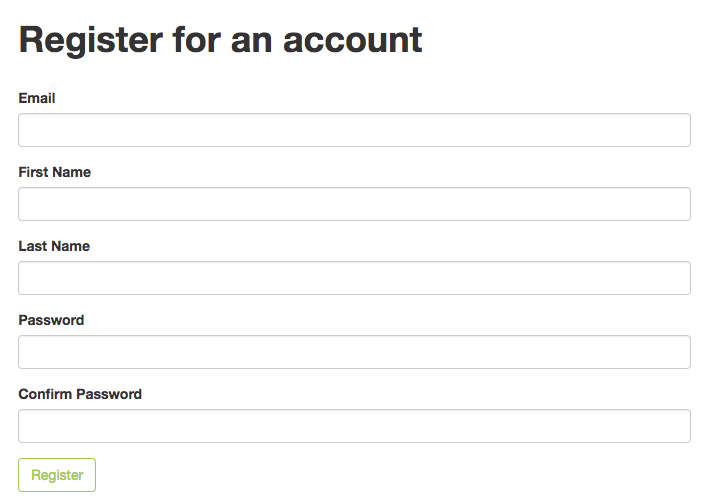
\includegraphics[width=\textwidth]{Figures/registration_page.png}
    \caption{Registration page}
    \label{fig:reg_page}
\end{figure}

\subsection{Login Page}
This is a simple login page. The user has to enter the Email ID and password and press Login. 
\begin{figure}[h]
    \centering
    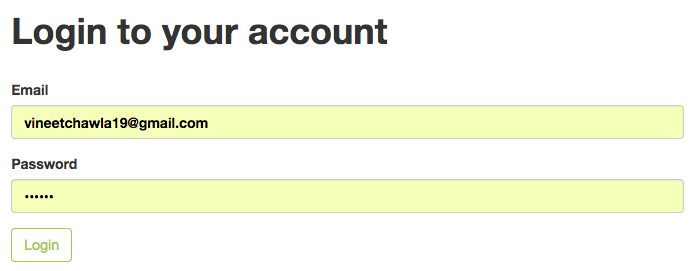
\includegraphics[width=\textwidth]{Figures/login_page.png}
    \caption{Login page}
    \label{fig:login_page}
\end{figure}

\subsection{Initial Dashboard}
The initial dashboard will be blank except for option for adding an insurance.
Once the user selects \textit{Add Insurance}, the user is redirected to Fight details webpage.
\begin{figure}[h]
    \centering
    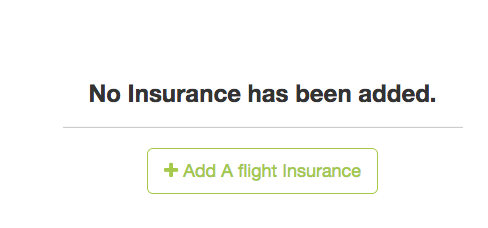
\includegraphics[width=\textwidth]{Figures/init_dashboard.png}
    \caption{Initial Dashboard}
    \label{fig:init_dash}
\end{figure}


\subsection{Header/Footer}
There are multiple values that are set dynamically in our header:
\begin{itemize}
    \item The rightmost field in the header is always \textit{Hi\,first\_name}.
    \item Once the user logs out, the Logout button is changed to login.
    \item The link to website's codebase in Github is also available in header.
\end{itemize}

\begin{figure}[h]
    \centering
    
\includegraphics[width=\textwidth]{Figures/header.png}
    \caption{Permanent Header. The rightmost field uses the user's first name.}
    \label{fig:header}
\end{figure}

\subsection{Flight Details}
The flight details page is the first part of the process of booking insurance for the user. Even though there are many fields visible to the user, only two fields can be filled by user input:
\begin{itemize}
    \item Flight ID
    \\This is a drop down list where as soon as the user enters two characters, the valid flight IDs will be automatically suggested.  On selecting a flight, automatically all the fields are populated with details of the flight selected. Only the suggest flight IDs will be considered valid for insurance. This auto completion is achieved using jQuery.
    \item Date
    \\ A simple date field for entering the date of the flight departure.
\end{itemize}
Once the user selects the Flight ID and date and presses \textit{Calcuate Insurance rates}, the user is redirected to the screen with insurance payout visibe.

\begin{figure}[h]
    \centering
    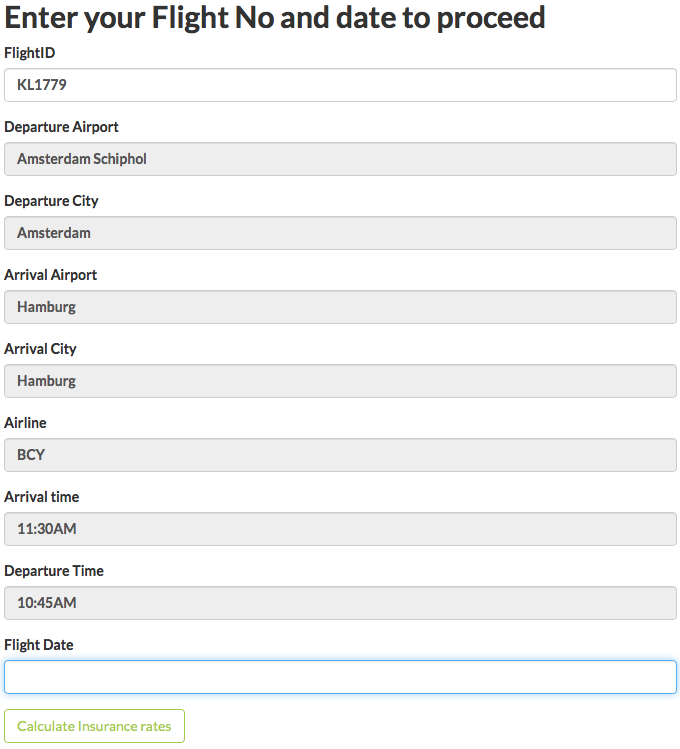
\includegraphics[width=\textwidth]{Figures/flight_details.png}
    \caption{Permanent Header. The rightmost field uses the user's first name.}
    \label{fig:flight_details}
\end{figure}

\subsection{Insurance Rates}
Even though we redirect from the previous page to this page, a whole lot of processing happens between the redirect page. We get all the flight details, we get the weather data for flight time at the selected date, fit the data in our model and predict the flight delay. Based on the flight delay, we calculate the insurance payout for each category of delay. Those rates are what displayed on this page. 
%%Add insurance screenshot
\\In a bid to be transparent, we present the user with payouts before they actually buy the insurance. If the user is satisfied with the rates he/she can move ahead and Buy insurance.

\subsection{Dashboard}
On buying the insurance, the user is redirected to the dashboard, but this time the user will have a new table on the dashboard. This table contains all the details of the insurance the user purchased along with the available blockchain anchoring proof, once available. Blockchain anchoring takes time due to fundamental design of how Bitcoin works. Hence the blockchain receipt is not initially available. That's why just after creating the insurance, your dashboard will have the blockchain status as unpublished as seen in figure \ref{fig:mid_dashboard}

\begin{figure}[h]
    \centering
    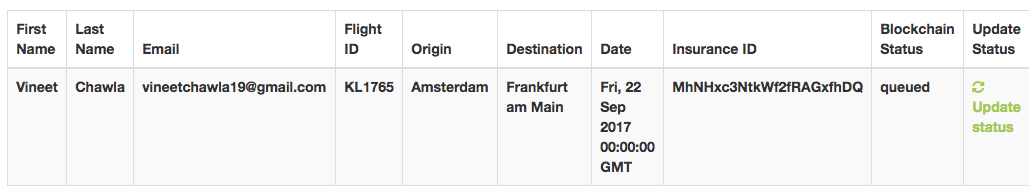
\includegraphics[width=\textwidth]{Figures/mid_dashboard.png}
    \caption{Insurance created but user details haven't been anchored to blockchain yet}
    \label{fig:mid_dashboard}
\end{figure}

The status update button is available on the dashboard, and pressing it refreshes the status. Within 10 minutes, we will have a blockchain status as complete and blockchain receipt in the box below the table as shown in figure \ref{fig:complete_dashboard}

\begin{figure}[h]
    \centering
    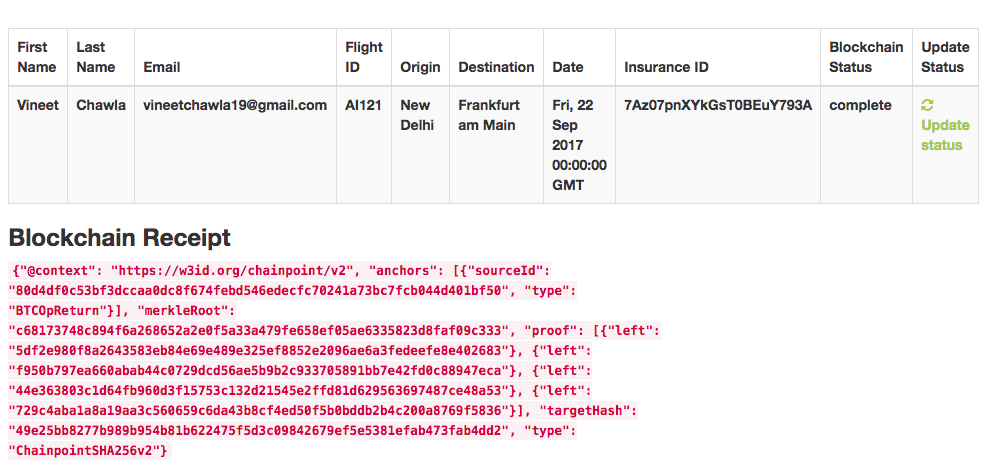
\includegraphics[width=\textwidth]{Figures/complete_dashboard.png}
    \caption{The Blockchain receipt is available and status has been updated}
    \label{fig:complete_dashboard}
\end{figure}

\subsection{Blockchain Receipt}
As shown in the last section, blockchain receipt is updated within ten minutes of creating the insurance. But what is blockchain receipt and what does it signify, we need to emphasise. Firstly the fields in blockchain receipt as show in table \ref{table:receipt}

\begin{table}[h!]
\centering
\begin{tabular}{||c c||} 
 \hline
 Name & Description  \\ [0.5ex] 
 \hline\hline
@context & the JSON-LD context for the receipt \\ 
\hline
type & receipt type definition specifying hash method and version \\
\hline
targetHash & hash value being anchored to the blockchain \\
\hline
merkleRoot	& merkle tree root value that is anchored to the blockchain \\
\hline
proof	& merkle proof establishing link from the targetHash to the merkleRoot \\
\hline
anchor-type	& anchor type definition specifying anchoring method (always bitcoin in our case \\
\hline
anchor-sourceId &	identifier, such as a transaction id, used to locate anchored data \\ [1ex]
 \hline
\end{tabular}
\caption{Different fields in blockchain receipt}
\label{table:receipt}
\end{table}

%%Explain significance of blockchain receipt


\section{Cloud Provider}
For cloud provider, the consideration was a web hosting company rather than cloud service providers like Amazon and Google. Hence we went with pythonanywhere.com. Instead of providing with empty VM's, it tries to automate most of the tedious work of setting up the web server. Even the database creation and initialisation is automated. 
The setup ensured that we don't have to manage our own web server or maintain a linux machine. Once we uploaded our code from github and initialised MySQL, the website was ready to go.
The tier chosen is just 5€ per website and scales dynamically, providing us with external internet connections too.

\section{Security Features}
Even though this is not a security project, the website security has been given utmost importance.
\begin{enumerate}
    \item HTTPS
    \\ We use a HTTPS certificate from Lets Encrypt to encrypt our connection.This maintains the privacy of connection and makes sure our connection doesn't leak any confidential data.
    \item Passwords are always stored as hashes. So in case of an attack, the attacker will never get to know the real passwords.
    \item There is not a single SQL query in the entire application. Creating SQL queries is handled by the API SQLAlchemy instead, we just pass parameters to the desired functions. Hence completely removing the possibility of SQL injection attacks
    \item Every user input is validated at the client side as well as server side
    \item Session variables are encrypted to prevent data leakage if website is accessed using public networks
\end{enumerate}

